\graphicspath{ {./JiaweiZhuang/} }

\begin{solution} 

To label the axis, we assume those parameter values (arbitrary choice, do not affect the shape of the curve):

\begin{align*}
a &= 2 \\
b &= 1 \\
Q &= -1
\end{align*}

The plots are shown in Fig \ref{fig:u(y)}, \ref{fig:u(z)}, \ref{fig:surf}.

\begin{figure}[H]
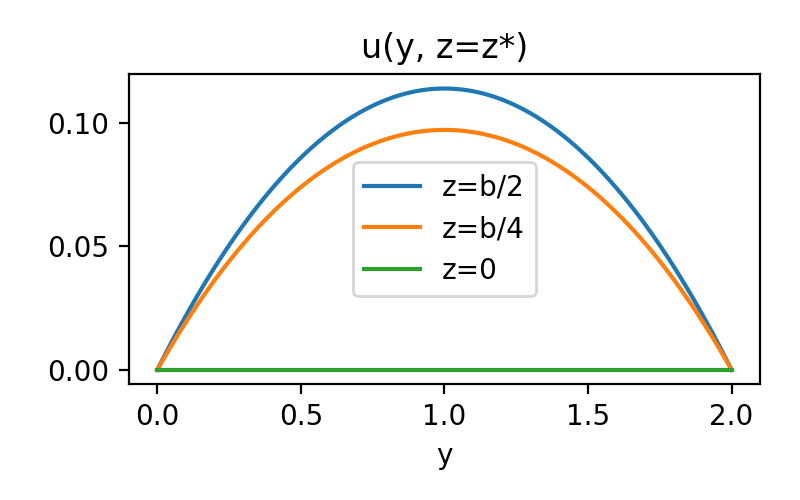
\includegraphics[scale=1]{u(y)}
\centering
\caption{u(y)}
\label{fig:u(y)}
\end{figure}

\begin{figure}[H]
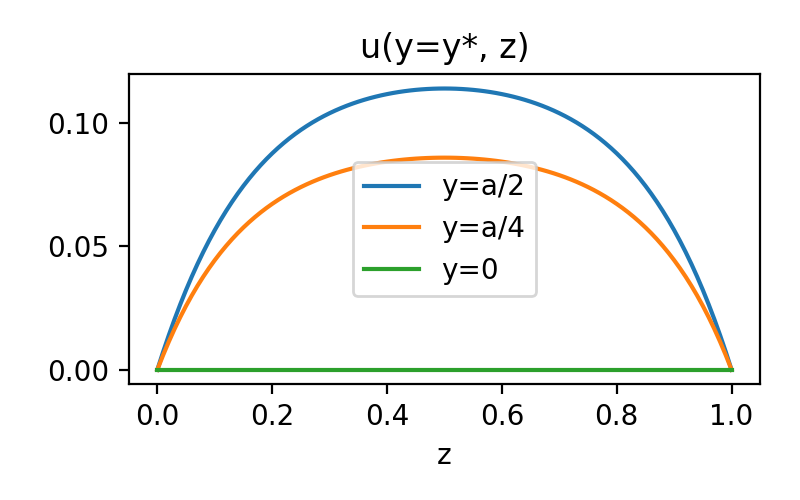
\includegraphics[scale=1]{u(z)}
\centering
\caption{u(z)}
\label{fig:u(z)}
\end{figure}

\end{solution} 

\begin{solution} 

\begin{figure}[H]
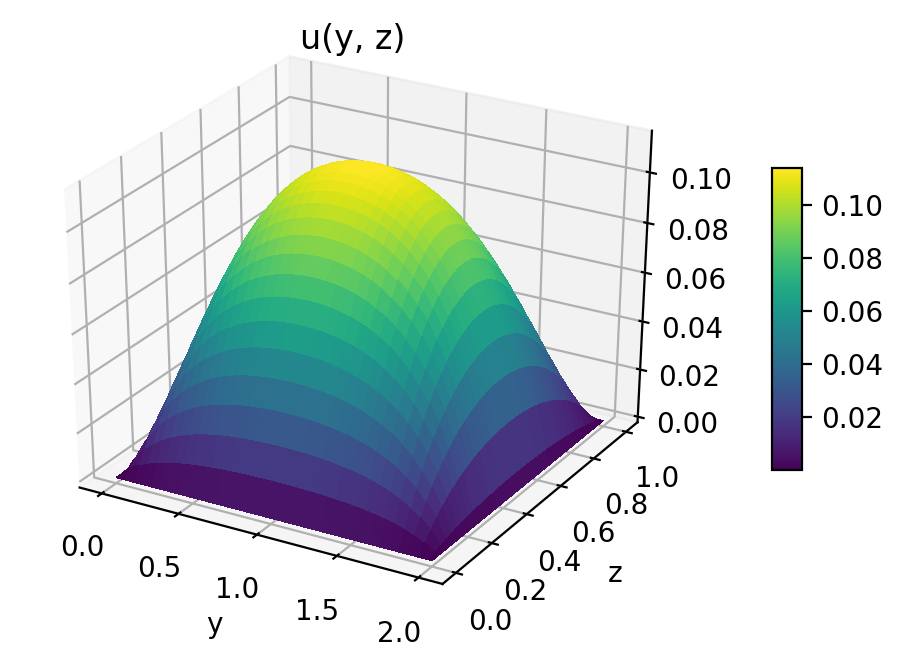
\includegraphics[scale=1]{surface_plot}
\centering
\caption{Surface plot of u(y, z)}
\label{fig:surf}
\end{figure}

See HW1P2\_plot.ipynb for the code generating the plots.

\end{solution} 